
%!TEX root = handout.tex

\newpage
\section{Isobaric analysis}
In the last chapters, we identified and quantified peptides in a label-free experiment. In this section, we would like to introduce a possible workflow for the analysis of isobaric data. We have prepared and copied this workflow to the USB sticks. Please import \directory{Workflows > Identification\_quantification\_isobaric\_MSstatsTMT } into KNIME via the menu entry \menu{File > Import KNIME workflow > Select file} and double-click the imported workflow in order to open it. Before you can execute the workflow, you again have to correct the locations of the files in the \KNIMENODE{Input Files} nodes (don't forget the one for the FASTA database inside the ``ID'' meta node). Try and run your workflow by executing all nodes at once.


\subsection{Workflow}
Let's have a look at the workflow (see Fig \ref{fig:isobaric_wf})

\begin{figure}[htbp]
  \centering
  
\includegraphics[width=0.95\textwidth]{graphics/isobaric/MSstatsTMT_export.png}
  \caption{Workflow for the analysis of isobaric data}
  \label{fig:isobaric_wf}
\end{figure}

\noindent The full analysis workflow can be found under\\
\directory{Workflows/Identification\_quantification\_isobaric\_MSstatsTMT}.

The workflow has three input nodes, the first for the experimental design to allow for MSstatsTMT compatible export (.tsv). The second for the .mzML files with the centroided spectra data from the isobaric labeling experiment and the last one for the .fasta database used for identification. The quantification (A) is performed using the \KNIMENODE{IsobaricAnalzyer}. The tool is able to extract and normalize quantiative information from TMT and iTRAQ data. The values can be assessed from centroided MS2 or MS3 spectra and isotopte correction is performed based on the specified correction matrix (as provided by the manufacturer). The identification (C) is performed as known from the previous chapters by using database search and a target-decoy database.

The workflow is performed peptide level (B, D, F, H), were the posterior error probability (PEP) estimation and FDR filtering is performed on PSM level for each file individually (B). Afterwards the identification (PSM) and quantiative information is combined using the \KNIMENODE{IDMapper}. After the processing of all available files, the intermediate results are aggregated (D) and can be exported via \KNIMENODE{MzTabExporter} (F) or further processed to obtain a MSstatsTMT
compatible version. Here, the R package MSstatsTMT can be used for further processing. \\

\subsubsection{Excursion MSstatsTMT}
The R package MSstatsTMT can be used for protein significance analysis in shotgun mass spectrometry-based proteomic experiments with tandem mass tag (TMT) labeling. MSstatsTMT provides functionality for two types of analysis: Protein summarization based on peptide quantification data and visualization and Model-based group comparison to detect significant changes in abundance. It depends on accurate feature detection, identification and quantification which can be performed e.g. by an OpenMS workflow. 

\noindent In general MSstatsTMT can be used for data processing \& visualization, as well as statistical modeling. Please see~\cite{Huang2020} and \url{http://msstats.org/msstatstmt/} for further information.

\subsubsection{Dataset}
We will illustrate the experimental design and the analysis on a subset of the Plubell 2017 dataset (~\cite{Plubell2017}; PRIDE: \url{https://www.ebi.ac.uk/pride/archive/projects/PXD005953}), which is a 10-plexed TMT labeling experiment to determine age and high fat diets specific proteome changes in mouse epididymal adipose tissue. It is a fairly complex multiplexing experiment with one technical replicate of 3 different TMT mixtures having 9 fractions each. 

\begin{figure}[htbp]
  \centering
  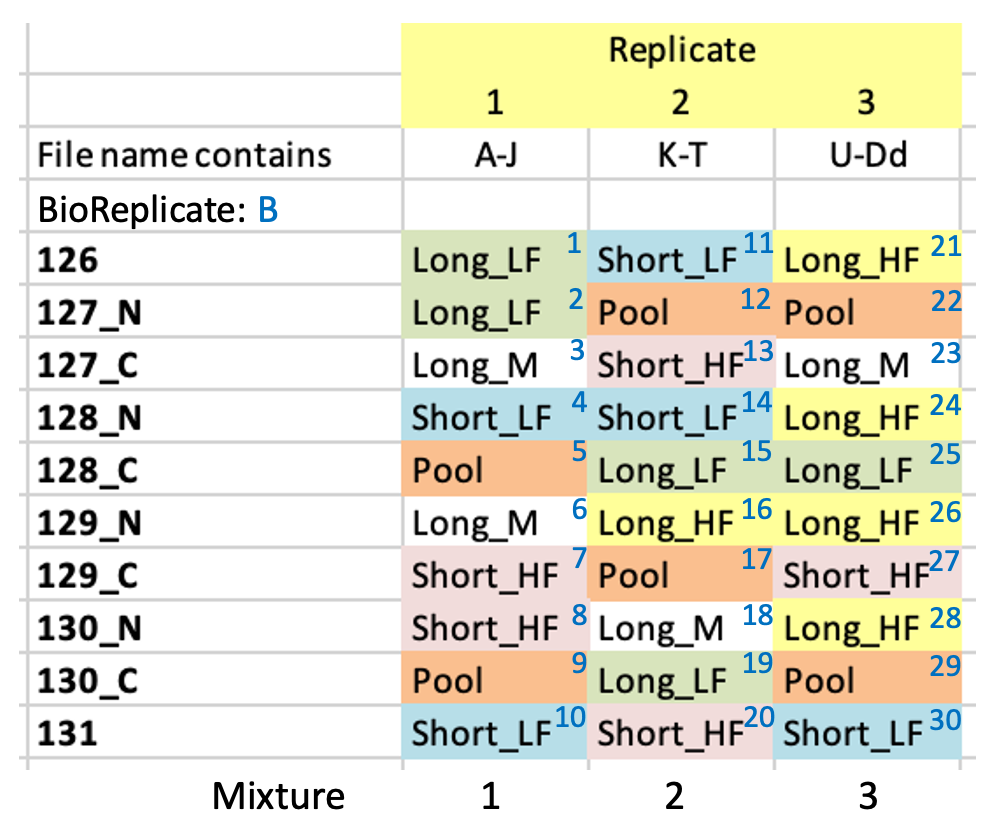
\includegraphics[width=0.95\textwidth]{graphics/isobaric/Dataset_MSstatsTMT.png}
  \caption{Dataset}
  \label{fig:isobaric_dataset_plubell}
\end{figure}

\subsection{Experimental Design (isobaric labeling)}
The experimental design for an isobaric labeling experiment is more complex than an LFQ experiment due to
the additional sources of variation coming from runs of different \textit{mixtures} which assign
peptide quantities (from reporter ions) to the different \textit{channels} of the labeling kit.
In this example we can omit the "TechRepMixture" column since every mixture was only analysed once on
the mass spectrometer. As there is only one "Condition" column allowed for MSstats, we use a concatenated
identifier for the combinations of time and treatment. We use "Norm" as a value to indicate channels
used for normalization (e.g. pooled channels). "Empty" could be used for empty channels (in case you had
more channels than samples).
For a great explanation of the different columns and the reasons for their existence,
see the following introductory video to MSstatsTMT:
\url{https://youtu.be/3CDnrQxGLbA}

\begin{table}[!ht]
\centering
\small
\begin{tabular}{0.95\textwidth}{lllll}
Spectra\_Filepath                         & Fraction           & Label                 & Fraction\_Group  & Sample    \\
PAMI-176\_Mouse\_A-J\_TMT\_14pctACN.mzML  & 1                  & 1                     & 1                & 1         \\
PAMI-176\_Mouse\_A-J\_TMT\_14pctACN.mzML  & 1                  & 2                     & 1                & 2         \\
PAMI-176\_Mouse\_A-J\_TMT\_14pctACN.mzML  & 1                  & 3                     & 1                & 3         \\
PAMI-176\_Mouse\_A-J\_TMT\_14pctACN.mzML  & 1                  & 4                     & 1                & 4         \\
PAMI-176\_Mouse\_A-J\_TMT\_14pctACN.mzML  & 1                  & 5                     & 1                & 5         \\
PAMI-176\_Mouse\_A-J\_TMT\_14pctACN.mzML  & 1                  & 6                     & 1                & 6         \\
PAMI-176\_Mouse\_A-J\_TMT\_14pctACN.mzML  & 1                  & 7                     & 1                & 7         \\
PAMI-176\_Mouse\_A-J\_TMT\_14pctACN.mzML  & 1                  & 8                     & 1                & 8         \\
PAMI-176\_Mouse\_A-J\_TMT\_14pctACN.mzML  & 1                  & 9                     & 1                & 9         \\
PAMI-176\_Mouse\_A-J\_TMT\_14pctACN.mzML  & 1                  & 10                    & 1                & 10        \\
PAMI-176\_Mouse\_K-T\_TMT\_14pctACN.mzML  & 1                  & 1                     & 2                & 11        \\
PAMI-176\_Mouse\_K-T\_TMT\_14pctACN.mzML  & 1                  & 2                     & 2                & 12        \\
PAMI-176\_Mouse\_K-T\_TMT\_14pctACN.mzML  & 1                  & 3                     & 2                & 13        \\
PAMI-176\_Mouse\_K-T\_TMT\_14pctACN.mzML  & 1                  & 4                     & 2                & 14        \\
PAMI-176\_Mouse\_K-T\_TMT\_14pctACN.mzML  & 1                  & 5                     & 2                & 15        \\
PAMI-176\_Mouse\_K-T\_TMT\_14pctACN.mzML  & 1                  & 6                     & 2                & 16        \\
PAMI-176\_Mouse\_K-T\_TMT\_14pctACN.mzML  & 1                  & 7                     & 2                & 17        \\
PAMI-176\_Mouse\_K-T\_TMT\_14pctACN.mzML  & 1                  & 8                     & 2                & 18        \\
PAMI-176\_Mouse\_K-T\_TMT\_14pctACN.mzML  & 1                  & 9                     & 2                & 19        \\
PAMI-176\_Mouse\_K-T\_TMT\_14pctACN.mzML  & 1                  & 10                    & 2                & 20        \\
PAMI-194\_Mouse\_U-Dd\_TMT\_14pctACN.mzML & 1                  & 1                     & 3                & 21        \\
PAMI-194\_Mouse\_U-Dd\_TMT\_14pctACN.mzML & 1                  & 2                     & 3                & 22        \\
PAMI-194\_Mouse\_U-Dd\_TMT\_14pctACN.mzML & 1                  & 3                     & 3                & 23        \\
PAMI-194\_Mouse\_U-Dd\_TMT\_14pctACN.mzML & 1                  & 4                     & 3                & 24        \\
PAMI-194\_Mouse\_U-Dd\_TMT\_14pctACN.mzML & 1                  & 5                     & 3                & 25        \\
PAMI-194\_Mouse\_U-Dd\_TMT\_14pctACN.mzML & 1                  & 6                     & 3                & 26        \\
PAMI-194\_Mouse\_U-Dd\_TMT\_14pctACN.mzML & 1                  & 7                     & 3                & 27        \\
PAMI-194\_Mouse\_U-Dd\_TMT\_14pctACN.mzML & 1                  & 8                     & 3                & 28        \\
PAMI-194\_Mouse\_U-Dd\_TMT\_14pctACN.mzML & 1                  & 9                     & 3                & 29        \\
PAMI-194\_Mouse\_U-Dd\_TMT\_14pctACN.mzML & 1                  & 10                    & 3                & 30        \\
\end{tabular}
\end{table}
\begin{table}[!ht]
\centering
\small
\begin{tabular}{0.95\textwidth}{lllll}
Sample                                    & MSstats\_Condition & MSstats\_BioReplicate & MSstats\_Mixture & LabelName \\
1                                         & Long\_LF           & 1                     & 1                & 126       \\
2                                         & Long\_LF           & 2                     & 1                & 127N      \\
3                                         & Long\_M            & 3                     & 1                & 127C      \\
4                                         & Short\_LF          & 4                     & 1                & 128N      \\
5                                         & Norm               & 5                     & 1                & 128C      \\
6                                         & Long\_M            & 6                     & 1                & 129N      \\
7                                         & Short\_HF          & 7                     & 1                & 129C      \\
8                                         & Short\_HF          & 8                     & 1                & 130N      \\
9                                         & Norm               & 9                     & 1                & 130C      \\
10                                        & Short\_LF          & 10                    & 1                & 131       \\
11                                        & Short\_LF          & 11                    & 2                & 126       \\
12                                        & Norm               & 12                    & 2                & 127N      \\
13                                        & Short\_HF          & 13                    & 2                & 127C      \\
14                                        & Short\_LF          & 14                    & 2                & 128N      \\
15                                        & Long\_LF           & 15                    & 2                & 128C      \\
16                                        & Long\_HF           & 16                    & 2                & 129N      \\
17                                        & Norm               & 17                    & 2                & 129C      \\
18                                        & Long\_M            & 18                    & 2                & 130N      \\
19                                        & Long\_LF           & 19                    & 2                & 130C      \\
20                                        & Short\_HF          & 20                    & 2                & 131       \\
21                                        & Long\_HF           & 21                    & 3                & 126       \\
22                                        & Norm               & 22                    & 3                & 127N      \\
23                                        & Long\_M            & 23                    & 3                & 127C      \\
24                                        & Long\_HF           & 24                    & 3                & 128N      \\
25                                        & Long\_LF           & 25                    & 3                & 128C      \\
26                                        & Long\_HF           & 26                    & 3                & 129N      \\
27                                        & Short\_HF          & 27                    & 3                & 129C      \\
28                                        & Long\_HF           & 28                    & 3                & 130N      \\
29                                        & Norm               & 29                    & 3                & 130C      \\
30                                        & Short\_LF          & 30                    & 3                & 131      
\end{tabular}
\end{table}

